\documentclass[titlepage, 11pt]{article}
\usepackage[utf8]{inputenc}     			% UTF8 encoding
\usepackage[margin=1in]{geometry}     		% margins 

\usepackage{hyperref} 						% href
\usepackage{graphicx}
\usepackage[font=small,labelfont=bf]{caption} % Required for specifying captions to tables and figures
\usepackage{multicol}


\title{
	\textbf{Mini Project 2: Deep Learning} \\
	Machine learning (CS582), MIU \thanks{Instructor: Anthony Sander}
}

\author{
    Baraa Mousa Noufal \and Ivan Krasowski Bissio
}
\date{\today}

\begin{document}
\maketitle
\tableofcontents

\begin{abstract}
	\addcontentsline{toc}{section}{Abstract}
	\begin{center}
    \begin{minipage}{0.85\textwidth}
        Machine Learning models are used to predict data of interest using known data as input.
        Deep Learning uses many-layers Neural Networks for approximating the predictor functions.
        When working with images as input, a special type of networks, called Convolutional Neural Networks, are most effective.\\
        The goal of this project is to implement a classifier for images,
        so to tell if each image is identifiable with one out of ten different labels.
        In the process, a secondary goal is to understand why one networks are more effective than others,
        so we build them for scratch, running to independent experiments with several attempts in each of them.
        Finally, we apply a distilled model\footnote{Knowledge Distillation: \href{https://keras.io/examples/vision/knowledge\_distillation/}{https://keras.io/examples/vision/knowledge\_distillation/}}
        looking to achieve similar performance with a simpler and lighter model.
    \end{minipage}
\end{center}
\end{abstract}

\section{About the Dataset}
The dataset we use is the \emph{CIFAR-10}\footnote{CIFAR-10 dataset: \href{https://keras.io/api/datasets/cifar10/}{https://keras.io/api/datasets/cifar10/}},
available for being downloaded directly using the Keras API.

\subsection{EDA: Exploratory Data Analysis}
The CIFAR-10 dataset consists of 60000 32x32 images in color (3 channels, RGB),
50000 for training and 10000 for testing. The output label for each image is a number
between 0 and 9, corresponding with the following table:
\begin{center}
    \begin{multicols}{2}
        \begin{itemize}
            \item 0 $\rightarrow$ airplane 
            \item 1 $\rightarrow$ automobile
            \item 2 $\rightarrow$ bird
            \item 3 $\rightarrow$ cat
            \item 4 $\rightarrow$ deer
            \item 5 $\rightarrow$ dog
            \item 6 $\rightarrow$ frog
            \item 7 $\rightarrow$ horse
            \item 8 $\rightarrow$ ship
            \item 9 $\rightarrow$ truck
        \end{itemize}
    \end{multicols}
\end{center}


\section{Experiment 1}
\subsection{Data Preparation}
For better estimations, augmented the data as such:
\begin{itemize}
    \item Normalized the color channels (input) values to be between 0-1
    \item One-Hot encoded the target labels
    \item Applied a data augmentor that applies random modifications to the data during training, namely small shifts and horizontal flips
\end{itemize}

\subsection{First Model (simple)}
The first model is an initial approach using a VGG inspired architecture.
\begin{center}
    \begin{verbatim}
        Model: "sequential_4"
_________________________________________________________________
Layer (type)                 Output Shape              Param #   
=================================================================
conv2d_26 (Conv2D)           (None, 32, 32, 32)        896       
_________________________________________________________________
conv2d_27 (Conv2D)           (None, 32, 32, 32)        9248      
_________________________________________________________________
max_pooling2d_13 (MaxPooling (None, 16, 16, 32)        0         
_________________________________________________________________
conv2d_28 (Conv2D)           (None, 16, 16, 64)        18496     
_________________________________________________________________
conv2d_29 (Conv2D)           (None, 16, 16, 64)        36928     
_________________________________________________________________
max_pooling2d_14 (MaxPooling (None, 8, 8, 64)          0         
_________________________________________________________________
conv2d_30 (Conv2D)           (None, 8, 8, 128)         73856     
_________________________________________________________________
conv2d_31 (Conv2D)           (None, 8, 8, 128)         147584    
_________________________________________________________________
max_pooling2d_15 (MaxPooling (None, 4, 4, 128)         0         
_________________________________________________________________
flatten_4 (Flatten)          (None, 2048)              0         
_________________________________________________________________
dense_8 (Dense)              (None, 128)               262272    
_________________________________________________________________
dense_9 (Dense)              (None, 10)                1290      
=================================================================
Total params: 550,570
Trainable params: 550,570
Non-trainable params: 0
_________________________________________________________________
    \end{verbatim}
\end{center}
This is a VGG-style network with 3 blocks compromised of 2 convolution layers and a pooling layer, followed by a dense fully connected layer for classification.
The ReLU\footnote{\href{https://machinelearningmastery.com/rectified-linear-activation-function-for-deep-learning-neural-networks/}{https://machinelearningmastery.com/rectified-linear-activation-function-for-deep-learning-neural-networks/}} activation function is used at each layer, and the loss function of the network is Cross Entropy\footnote{\href{https://www.tensorflow.org/api\_docs/python/tf/keras/losses/CategoricalCrossentropy}{https://www.tensorflow.org/api\_docs/python/tf/keras/losses/CategoricalCrossentropy}}
The network is optimized using the Adam algorithm\footnote{\href{https://keras.io/api/optimizers/adam/}{https://keras.io/api/optimizers/adam/}}.
This model gave an accuracy of about 83% after 50 epochs, but the learning curve indicates overfitting happening early on.
\begin{center}
    \captionsetup{type=figure}
    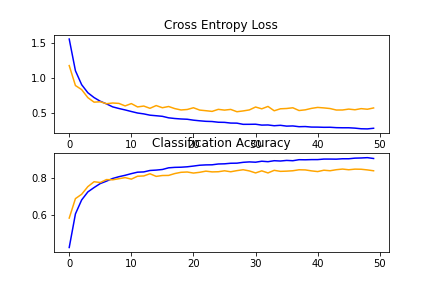
\includegraphics[width=250px]{sections/exp-2/images/initial-plot.png}
    \captionof{figure}{Experiment 2 - Model 1 - Cross Entropy Loss \& Classification Accuracy}
\end{center}
The problem of overfitting will be addressed the second model, by introducing dropout in the network, we will also attempt to increase prediction accuracy by introducing batch normalization and another dense classification layer.


\subsection{Second Model (complex)}
The second model is an improved version using roughly the same architecture as the first, but adding dropout to reduce overfitting, batch normalization and another dense fully connected layer.
\begin{center}
    \begin{verbatim}
    Model: "sequential_3"
    _________________________________________________________________
    Layer (type)                 Output Shape              Param #   
    =================================================================
    conv2d_18 (Conv2D)           (None, 32, 32, 32)        896       
    _________________________________________________________________
    batch_normalization_12 (Batc (None, 32, 32, 32)        128       
    _________________________________________________________________
    conv2d_19 (Conv2D)           (None, 32, 32, 32)        9248      
    _________________________________________________________________
    batch_normalization_13 (Batc (None, 32, 32, 32)        128       
    _________________________________________________________________
    max_pooling2d_9 (MaxPooling2 (None, 16, 16, 32)        0         
    _________________________________________________________________
    dropout_8 (Dropout)          (None, 16, 16, 32)        0         
    _________________________________________________________________
    conv2d_20 (Conv2D)           (None, 16, 16, 64)        18496     
    _________________________________________________________________
    batch_normalization_14 (Batc (None, 16, 16, 64)        256       
    _________________________________________________________________
    conv2d_21 (Conv2D)           (None, 16, 16, 64)        36928     
    _________________________________________________________________
    batch_normalization_15 (Batc (None, 16, 16, 64)        256       
    _________________________________________________________________
    max_pooling2d_10 (MaxPooling (None, 8, 8, 64)          0         
    _________________________________________________________________
    dropout_9 (Dropout)          (None, 8, 8, 64)          0         
    _________________________________________________________________
    conv2d_22 (Conv2D)           (None, 8, 8, 128)         73856     
    _________________________________________________________________
    batch_normalization_16 (Batc (None, 8, 8, 128)         512       
    _________________________________________________________________
    conv2d_23 (Conv2D)           (None, 8, 8, 128)         147584    
    _________________________________________________________________
    batch_normalization_17 (Batc (None, 8, 8, 128)         512       
    _________________________________________________________________
    max_pooling2d_11 (MaxPooling (None, 4, 4, 128)         0         
    _________________________________________________________________
    dropout_10 (Dropout)         (None, 4, 4, 128)         0         
    _________________________________________________________________
    flatten_3 (Flatten)          (None, 2048)              0         
    _________________________________________________________________
    dense_8 (Dense)              (None, 128)               262272    
    _________________________________________________________________
    dense_9 (Dense)              (None, 64)                8256      
    _________________________________________________________________
    dropout_11 (Dropout)         (None, 64)                0         
    _________________________________________________________________
    dense_10 (Dense)             (None, 10)                650       
    =================================================================
    Total params: 559,978
    Trainable params: 559,082
    Non-trainable params: 896
    _________________________________________________________________
    \end{verbatim}
\end{center}
This is a VGG-style network with 3 blocks compromised of 2 convolution layers and a pooling layer, followed by a dense fully connected layer for classification.
The ReLU\footnote{\href{https://machinelearningmastery.com/rectified-linear-activation-function-for-deep-learning-neural-networks/}{https://machinelearningmastery.com/rectified-linear-activation-function-for-deep-learning-neural-networks/}} activation function is used at each layer, and the loss function of the network is Cross Entropy\footnote{\href{https://www.tensorflow.org/api\_docs/python/tf/keras/losses/CategoricalCrossentropy}{https://www.tensorflow.org/api\_docs/python/tf/keras/losses/CategoricalCrossentropy}}
Batch Normalization is applied after each convolution layer.
Increasing dropout starting at 20\% after the first convolution block going up to 50\% at the final dense layer is applied.
This model resulted in an improved 85\% accuracy after 50 epochs, and as indicated by the learning curve, it can definitely benefit from more training epochs, and the overfitting problem from the previous model is now gone.
\begin{center}
    \captionsetup{type=figure}
    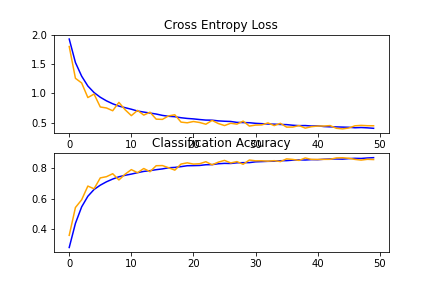
\includegraphics[width=250px]{sections/exp-2/images/improved-plot.png}
    \captionof{figure}{Model 1 - Cross Entropy Loss \& Classification Accuracy}
\end{center}


\subsection{Distiller}
Finally, we try to go one step further with the network, making it simpler without losing much performance.
Given that we have a trained model with over 75\%, we can use \emph{knowledge distillation}
\footnote{"Knowledge Distillation and Student-Teacher Learning for Visual Intelligence: A Review and
New Outlooks", available at \href{https://arxiv.org/pdf/2004.05937.pdf}{https://arxiv.org/pdf/2004.05937.pdf}}
on it, defining its role as a \emph{teacher} and creating a much simpler \emph{student} model.\\
Teacher network:
\begin{center}
    \begin{verbatim}
        Model: "teacher"
        _________________________________________________________________
        Layer (type)                 Output Shape              Param #   
        =================================================================
        conv2d (Conv2D)              (None, 32, 32, 32)        320       
        _________________________________________________________________
        batch_normalization (BatchNo (None, 32, 32, 32)        128       
        _________________________________________________________________
        conv2d_1 (Conv2D)            (None, 32, 32, 32)        9248      
        _________________________________________________________________
        batch_normalization_1 (Batch (None, 32, 32, 32)        128       
        _________________________________________________________________
        max_pooling2d (MaxPooling2D) (None, 16, 16, 32)        0         
        _________________________________________________________________
        dropout (Dropout)            (None, 16, 16, 32)        0         
        _________________________________________________________________
        conv2d_2 (Conv2D)            (None, 16, 16, 64)        18496     
        _________________________________________________________________
        batch_normalization_2 (Batch (None, 16, 16, 64)        256       
        _________________________________________________________________
        conv2d_3 (Conv2D)            (None, 16, 16, 64)        36928     
        _________________________________________________________________
        batch_normalization_3 (Batch (None, 16, 16, 64)        256       
        _________________________________________________________________
        max_pooling2d_1 (MaxPooling2 (None, 8, 8, 64)          0         
        _________________________________________________________________
        dropout_1 (Dropout)          (None, 8, 8, 64)          0         
        _________________________________________________________________
        conv2d_4 (Conv2D)            (None, 8, 8, 128)         73856     
        _________________________________________________________________
        batch_normalization_4 (Batch (None, 8, 8, 128)         512       
        _________________________________________________________________
        conv2d_5 (Conv2D)            (None, 8, 8, 128)         147584    
        _________________________________________________________________
        batch_normalization_5 (Batch (None, 8, 8, 128)         512       
        _________________________________________________________________
        max_pooling2d_2 (MaxPooling2 (None, 4, 4, 128)         0         
        _________________________________________________________________
        dropout_2 (Dropout)          (None, 4, 4, 128)         0         
        _________________________________________________________________
        flatten (Flatten)            (None, 2048)              0         
        _________________________________________________________________
        dense (Dense)                (None, 128)               262272    
        _________________________________________________________________
        dense_1 (Dense)              (None, 10)                1290      
        =================================================================
        Total params: 551,786
        Trainable params: 550,890
        Non-trainable params: 896
        _________________________________________________________________
    \end{verbatim}
\end{center}
Student network:
\begin{center}
    \begin{verbatim}
        Model: "student"
        _________________________________________________________________
        Layer (type)                 Output Shape              Param #   
        =================================================================
        conv2d_6 (Conv2D)            (None, 32, 32, 32)        320       
        _________________________________________________________________
        batch_normalization_6 (Batch (None, 32, 32, 32)        128       
        _________________________________________________________________
        conv2d_7 (Conv2D)            (None, 32, 32, 32)        9248      
        _________________________________________________________________
        batch_normalization_7 (Batch (None, 32, 32, 32)        128       
        _________________________________________________________________
        max_pooling2d_3 (MaxPooling2 (None, 16, 16, 32)        0         
        _________________________________________________________________
        dropout_3 (Dropout)          (None, 16, 16, 32)        0         
        _________________________________________________________________
        flatten_1 (Flatten)          (None, 8192)              0         
        _________________________________________________________________
        dense_2 (Dense)              (None, 10)                81930     
        =================================================================
        Total params: 91,754
        Trainable params: 91,626
        Non-trainable params: 128
        _________________________________________________________________
    \end{verbatim}
\end{center}
For the implementation, we use as a guide the Keras documentation.\footnote{\href{https://keras.io/examples/vision/knowledge\_distillation/}{https://keras.io/examples/vision/knowledge\_distillation/}}
The experiment consists in training the student model both from the input and from the weights learned by the teacher model.
In order to achieve this, the loss function to minimize by the student, other than the Cross Entropy for the teacher, is KL Divergence
\footnote{\href{https://www.tensorflow.org/api\_docs/python/tf/keras/losses/KLDivergence}{https://www.tensorflow.org/api\_docs/python/tf/keras/losses/KLDivergence}},
which considers both results and leads the student to learn from them.\\
Unfortunately, our experimenting results are not very successful, given that training our student model for itself gives us almost the same results than the distilled version.
We tried different values for the distiller's parameters (temperature, alpha), as well as different layers dispositions for the student, always with similar results
(even getting worse accuracies, but both alike). Given a teacher with approximately 75\% accuracy, we obtain a student with approximately 58\% accuracy:
\begin{center}
    \captionsetup{type=figure}
    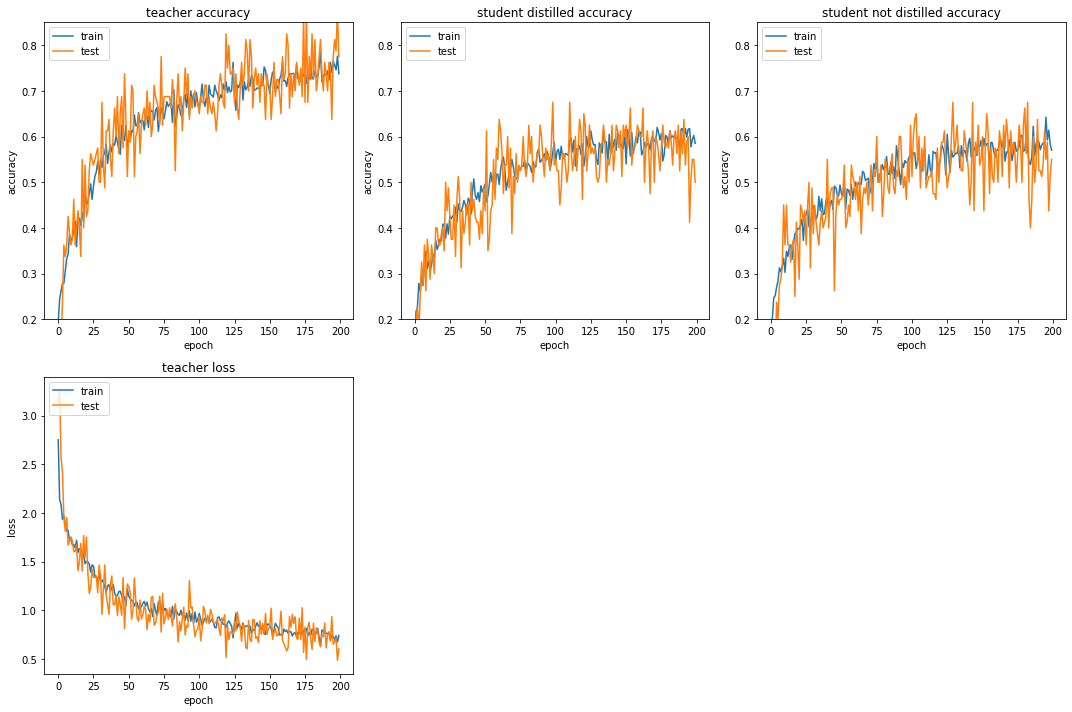
\includegraphics[width=400px]{sections/exp-1/images/distiller-acc.png}
    \captionof{figure}{Distilling - Loss \& Accuracy}
\end{center}


\section{Experiment 2}
\subsection{Data Preparation}
For better estimations, augmented the data as such:
\begin{itemize}
    \item Normalized the color channels (input) values to be between 0-1
    \item One-Hot encoded the target labels
    \item Applied a data augmentor that applies random modifications to the data during training, namely small shifts and horizontal flips
\end{itemize}

\subsection{First Model (initial)}
The first model is an initial approach using a VGG inspired architecture.
\begin{center}
    \begin{verbatim}
        Model: "sequential_4"
_________________________________________________________________
Layer (type)                 Output Shape              Param #   
=================================================================
conv2d_26 (Conv2D)           (None, 32, 32, 32)        896       
_________________________________________________________________
conv2d_27 (Conv2D)           (None, 32, 32, 32)        9248      
_________________________________________________________________
max_pooling2d_13 (MaxPooling (None, 16, 16, 32)        0         
_________________________________________________________________
conv2d_28 (Conv2D)           (None, 16, 16, 64)        18496     
_________________________________________________________________
conv2d_29 (Conv2D)           (None, 16, 16, 64)        36928     
_________________________________________________________________
max_pooling2d_14 (MaxPooling (None, 8, 8, 64)          0         
_________________________________________________________________
conv2d_30 (Conv2D)           (None, 8, 8, 128)         73856     
_________________________________________________________________
conv2d_31 (Conv2D)           (None, 8, 8, 128)         147584    
_________________________________________________________________
max_pooling2d_15 (MaxPooling (None, 4, 4, 128)         0         
_________________________________________________________________
flatten_4 (Flatten)          (None, 2048)              0         
_________________________________________________________________
dense_8 (Dense)              (None, 128)               262272    
_________________________________________________________________
dense_9 (Dense)              (None, 10)                1290      
=================================================================
Total params: 550,570
Trainable params: 550,570
Non-trainable params: 0
_________________________________________________________________
    \end{verbatim}
\end{center}
This is a VGG-style network with 3 blocks compromised of 2 convolution layers and a pooling layer, followed by a dense fully connected layer for classification.
The ReLU\footnote{\href{https://machinelearningmastery.com/rectified-linear-activation-function-for-deep-learning-neural-networks/}{https://machinelearningmastery.com/rectified-linear-activation-function-for-deep-learning-neural-networks/}} activation function is used at each layer, and the loss function of the network is Cross Entropy\footnote{\href{https://www.tensorflow.org/api\_docs/python/tf/keras/losses/CategoricalCrossentropy}{https://www.tensorflow.org/api\_docs/python/tf/keras/losses/CategoricalCrossentropy}}
The network is optimized using the Adam algorithm\footnote{\href{https://keras.io/api/optimizers/adam/}{https://keras.io/api/optimizers/adam/}}.
This model gave an accuracy of about 83% after 50 epochs, but the learning curve indicates overfitting happening early on.
\begin{center}
    \captionsetup{type=figure}
    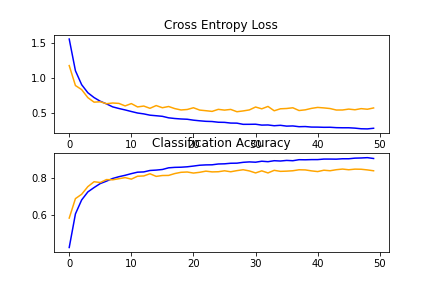
\includegraphics[width=250px]{sections/exp-2/images/initial-plot.png}
    \captionof{figure}{Experiment 2 - Model 1 - Cross Entropy Loss \& Classification Accuracy}
\end{center}
The problem of overfitting will be addressed the second model, by introducing dropout in the network, we will also attempt to increase prediction accuracy by introducing batch normalization and another dense classification layer.


\subsection{Second Model (improved)}
The second model is an improved version using roughly the same architecture as the first, but adding dropout to reduce overfitting, batch normalization and another dense fully connected layer.
\begin{center}
    \begin{verbatim}
    Model: "sequential_3"
    _________________________________________________________________
    Layer (type)                 Output Shape              Param #   
    =================================================================
    conv2d_18 (Conv2D)           (None, 32, 32, 32)        896       
    _________________________________________________________________
    batch_normalization_12 (Batc (None, 32, 32, 32)        128       
    _________________________________________________________________
    conv2d_19 (Conv2D)           (None, 32, 32, 32)        9248      
    _________________________________________________________________
    batch_normalization_13 (Batc (None, 32, 32, 32)        128       
    _________________________________________________________________
    max_pooling2d_9 (MaxPooling2 (None, 16, 16, 32)        0         
    _________________________________________________________________
    dropout_8 (Dropout)          (None, 16, 16, 32)        0         
    _________________________________________________________________
    conv2d_20 (Conv2D)           (None, 16, 16, 64)        18496     
    _________________________________________________________________
    batch_normalization_14 (Batc (None, 16, 16, 64)        256       
    _________________________________________________________________
    conv2d_21 (Conv2D)           (None, 16, 16, 64)        36928     
    _________________________________________________________________
    batch_normalization_15 (Batc (None, 16, 16, 64)        256       
    _________________________________________________________________
    max_pooling2d_10 (MaxPooling (None, 8, 8, 64)          0         
    _________________________________________________________________
    dropout_9 (Dropout)          (None, 8, 8, 64)          0         
    _________________________________________________________________
    conv2d_22 (Conv2D)           (None, 8, 8, 128)         73856     
    _________________________________________________________________
    batch_normalization_16 (Batc (None, 8, 8, 128)         512       
    _________________________________________________________________
    conv2d_23 (Conv2D)           (None, 8, 8, 128)         147584    
    _________________________________________________________________
    batch_normalization_17 (Batc (None, 8, 8, 128)         512       
    _________________________________________________________________
    max_pooling2d_11 (MaxPooling (None, 4, 4, 128)         0         
    _________________________________________________________________
    dropout_10 (Dropout)         (None, 4, 4, 128)         0         
    _________________________________________________________________
    flatten_3 (Flatten)          (None, 2048)              0         
    _________________________________________________________________
    dense_8 (Dense)              (None, 128)               262272    
    _________________________________________________________________
    dense_9 (Dense)              (None, 64)                8256      
    _________________________________________________________________
    dropout_11 (Dropout)         (None, 64)                0         
    _________________________________________________________________
    dense_10 (Dense)             (None, 10)                650       
    =================================================================
    Total params: 559,978
    Trainable params: 559,082
    Non-trainable params: 896
    _________________________________________________________________
    \end{verbatim}
\end{center}
This is a VGG-style network with 3 blocks compromised of 2 convolution layers and a pooling layer, followed by a dense fully connected layer for classification.
The ReLU\footnote{\href{https://machinelearningmastery.com/rectified-linear-activation-function-for-deep-learning-neural-networks/}{https://machinelearningmastery.com/rectified-linear-activation-function-for-deep-learning-neural-networks/}} activation function is used at each layer, and the loss function of the network is Cross Entropy\footnote{\href{https://www.tensorflow.org/api\_docs/python/tf/keras/losses/CategoricalCrossentropy}{https://www.tensorflow.org/api\_docs/python/tf/keras/losses/CategoricalCrossentropy}}
Batch Normalization is applied after each convolution layer.
Increasing dropout starting at 20\% after the first convolution block going up to 50\% at the final dense layer is applied.
This model resulted in an improved 85\% accuracy after 50 epochs, and as indicated by the learning curve, it can definitely benefit from more training epochs, and the overfitting problem from the previous model is now gone.
\begin{center}
    \captionsetup{type=figure}
    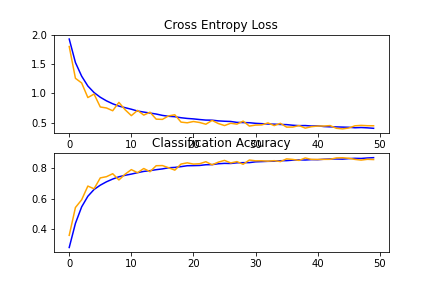
\includegraphics[width=250px]{sections/exp-2/images/improved-plot.png}
    \captionof{figure}{Model 1 - Cross Entropy Loss \& Classification Accuracy}
\end{center}




\clearpage
\section{Conclusion}
% Different approaches, metrics, algorithms for the same data can gives us very diverse recommendations, depending on our interests.
% From this project, we understand that the important part of getting an accurate recommender is interpreting well our data, and what we want from it
% (for instance, going from a simple general demographic recommendation up to a personalized recommendation based in our previous preferences and the collaboration of others).

% \subsection*{Future Work}
% \begin{itemize}
%     % \item As mentioned on the corresponding section, the \emph{weighted average rating} is a metric developed by IMDb, and found to be useful for them. There might be different metrics with better results for our demographic filtering, still waiting for us to try them.
%     % \item Similarly, the Content-based recommender might be improved by adding/removing features to the similarity calculation, or even changing the coefficient. To be certain of this, experimentation is required.
%     % \item Regarding the Neural Collaborative approach, train the model with a larger dataset, and check whether the layers disposition or the hyperparameters can be tweaked into a better performance.
%     % \item With the same idea, the response times for the web-service can be optimized, either by improving the caching system or even the algorithm.
% \end{itemize}


\end{document}
